\documentclass[a4paper, 10pt]{article}

\usepackage[english]{babel}
\usepackage[T1]{fontenc}
\usepackage[utf8]{inputenc}
\usepackage{textcomp}

\setlength{\marginparwidth}{2cm}

\usepackage{comment}
\usepackage{todonotes}

\usepackage{xcolor}
\usepackage{graphicx}
\graphicspath{ {./img/} }

\usepackage{hyperref}

\title{Homework Assignment N°1}
\author{Thibault Douzon\\Rajavarman Mathivanan}
\date{September 4th, 2018}


\begin{document}
\maketitle

\pagebreak

\tableofcontents
\pagebreak

\section{Exercise 1: Geometry}
\subsection{Part a}
We have:
\\
$$
w_0 + 3w_1 + w_2 = 0
$$
$$
w_0 - w_1 + 2w_2 = 0
$$
\\
Normalize by $w_2$ it gives
\\
$$
W_0 + 3W_1 = -1
$$
$$
W_0 - W_1 = -2
$$
Where $W_0 = \frac{w_0}{w_2}$ and $W_1 = \frac{w_1}{w_2}$
\\
Cramer's rule gives us the results:
$$
W_0 = \frac{(-1 \times -1) - (3 \times -2)}{(1 \times -1) - (1 \times 3)}
    = -\frac{7}{4}
$$
$$
W_1 = \frac{(1 \times -2) - (-1 \times 1)}{(1 \times -1) - (1 \times 3)}
    = \frac{1}{4}
$$
Thus, we can chose $w_2 = 1$ and then
$$
w_0 = - \frac{7}{4}
$$
$$
w_1 = \frac{1}{4}
$$
$$
w_2 = 1
$$

We can check our first system is solved with this solution.
Hence the equation of the line is the following:
$$
- \frac{7}{4} + \frac{x_1}{4} + x_2 = 0
$$ 

\subsection{Part b}
Our figure is the following:
\\
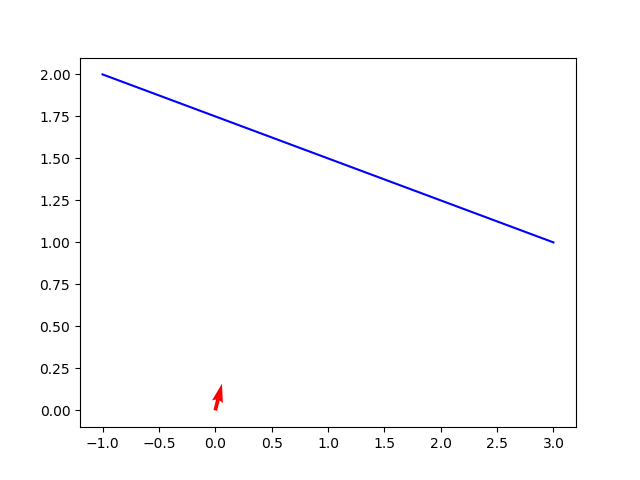
\includegraphics[scale=0.6]{ex1_partb.png}

\subsection{Part c}
The point $(4, 3)$ is in the positive side of the line, the most simple «proof» is this plot:
\\
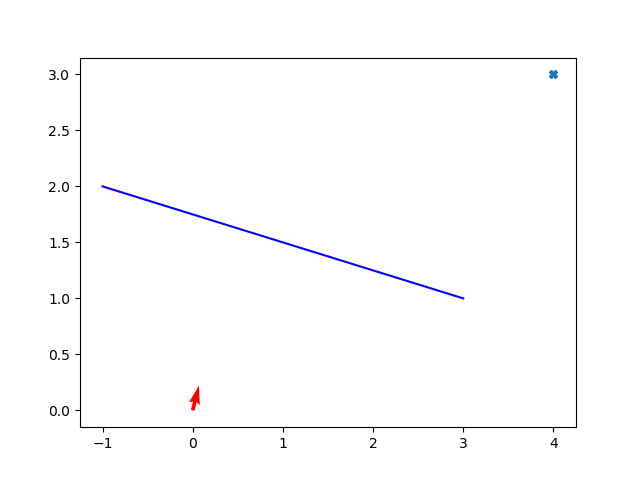
\includegraphics[scale=0.6]{ex1_partc.png}
\\
It shows our point «above» the blue line, hence it is in the positive side of the line.
For this point, because we saw it was on the positive side, $w_0 + w_1x_1+w_2x_2$ should give a positive result.
$$
-\frac{7}{4}+\frac{4}{4}+3 = \frac{9}{4} > 0
$$

\subsection{Part d}
First we must notice that $(w_1, w_2)$ is orthogonal to our line.
To figure out the direction vector of the line, we can rewrite its equation like this
$$
-w_1x - w_0 = w_2y
$$
Hence its direction vector is $(w_2, -w_1)$ and now we can proove that
$(w_1, w_2)$ is orthogonal to the line by showing that 
$$
(w_1, w_2) \cdot (w_2, -w_1) = 0
$$

Now we know the perpendicular direction to the line, we can compute the distance between the point and the line.



$$
d_{line}(P) = \left\vert [(x_1, x_2) - (3, 1)] \cdot (w_1, w_2) \right\vert / \left\Vert (w_1, w_2) \right\Vert 
$$

$$
d_{line}(P) = \left\vert x_1w_1 + x_2 w_2 - 3w_1 - 1w_2\right\vert / \left\Vert (w_1, w_2) \right\Vert 
$$
Or because $w_0 + 3w_1 + 1w_2 = 0$ ($(3, 1)$ is on the line) we can add $w_0 + 3w_1 + 1w_2$ without changing the value.
Hence:
$$
d_{line}(P) = \frac{\left\vert w_0+x_1w_1+x_2w_2\right\vert}{\left\Vert(w_1, w_2)\right\Vert}
$$

\subsection{Part e}
We use what we learned from part d:

$$
d_{line}((0, 0)) = \frac{\left\vert w_0\right\vert}{\left\Vert(w_1, w_2)\right\Vert}
$$
Hence we have
$$
d_{line}((0, 0)) = \frac{\left\vert w_0\right\vert}{\sqrt{{w_1}^2 + {w_2}^2}} = \frac{\frac{7}{4}}{\sqrt{{\frac{1}{4}}^2+1}} \approx 1.7
$$

\section{Exercice 2: Calculus}
$$
\sigma(y) = \frac{1}{1+e^{-y}}
$$
\subsection{Part a}
Calculus says $\left(\frac{u}{v}\right)^{\prime} = \frac{u^{\prime}v - uv^{\prime}}{v^2}$, then:
$$
\sigma^{\prime}(y) = \frac{e^{-y}}{\left(1+e^{-y}\right)^2}
$$
$$
\sigma^{\prime}(y) = \frac{(1 + e^{-y}) - 1}{\left(1+e^{-y}\right)^2}
$$
$$
\sigma^{\prime}(y) = \sigma(y) \times \frac{(1 + e^{-y}) - 1}{1+e^{-y}}
$$
$$
\sigma^{\prime}(y) = \sigma(y) \times (1 - \sigma(y))
$$

\subsection{Part b}
We know that $\lim_{y\to\infty} e^{-y} = 0$ thus because the denominator does not tend to zero:
$$
\lim_{y\to\infty} \sigma(y) = \frac{1}{1+\lim_{y\to\infty}e^{-y}} = 1
$$
and now we know the limit exists and its value:
$$
\lim_{y\to\infty}\sigma^{\prime}(y) = \lim_{y\to\infty} \sigma(y) \times (1-\sigma(y)) = 1 \times (1-1) = 0
$$

\subsection{Part c}

Hey this a new line
\end{document}